\documentclass[conference]{IEEEtran}

\usepackage{cite}
\usepackage{amsmath,amssymb,amsfonts}
\usepackage{verbatim} % um viele zeilen auszukommentieren
\usepackage{algorithmic}
\usepackage{listings}
\usepackage{listings}
\lstset{
	language=Python,
	basicstyle=\ttfamily\small,
	aboveskip={1.0\baselineskip},
	belowskip={1.0\baselineskip},
	columns=fixed,
	extendedchars=true,
	breaklines=true,
	tabsize=4,
	frame=lines,
	showtabs=false,
	showspaces=false,
	showstringspaces=false,
	keywordstyle=\color[rgb]{0.627,0.126,0.941},
	commentstyle=\color[rgb]{0.133,0.545,0.133},
	stringstyle=\color[rgb]{01,0,0},
	numbers=left,
	numberstyle=\small,
	stepnumber=1,
	numbersep=10pt,
	captionpos=t,
	escapeinside={\%*}{*)}
}


\usepackage{graphicx}
\usepackage[ngerman]{babel}		% Achtung umlaut 
\usepackage[utf8]{inputenc}       % UTF-8 ist wichtig,  ASCII hat nicht alle Schriftzeichen  
\usepackage{textcomp}
\usepackage{xcolor}
\usepackage{dirtytalk} % nein, nicht was du denkst.  Packet hilft  gegen verschluckte gänsefüschen
\def\BibTeX{{\rm B\kern-.05em{\sc i\kern-.025em b}\kern-.08em T\kern-.1667em\lower.7ex\hbox{E}\kern-.125emX}}
\begin{document}
	
	\title{Projekt rosBerry *\\
		{\footnotesize \textsuperscript{*}Ein Autonomer Roboter auf der Basis von ROS , gebaut aus einem Modeauto Chassis mit Maker Elektronik}}
	
	\author{\IEEEauthorblockN{1\textsuperscript{st} Welter, Heike}
		\IEEEauthorblockA{\textit{Hochschule Mannheim} \\
			email address 1630298@stud.hs-mannheim.de}%
		\and
		\IEEEauthorblockN{2\textsuperscript{nd} Matteis, Steffen}
		\IEEEauthorblockA{\textit{Hochschule Mannheim} \\
			email address}%noch 
		\and
		\IEEEauthorblockN{3\textsuperscript{rd}Barsalou Marie }
		\IEEEauthorblockA{\textit{Hochschule Mannheim} \\
			email address 1611347@stud.hs-mannheim.de}
	}
	
	\maketitle
	
	\begin{abstract}
		Ziel von Projekt rosBerry besteht darin einen kleinen, schnellen aber dennoch preisgünstigen Roboter aus leicht verfügbaren Standartbauteilen zu Bauen. Zusätzlich soll er mit dem Robot Operating System Betrieben werden und mit einer Künstlichen Intelligenz versehen. Der Roboter soll einen optischen Marker erkennen und darauf zufahren. Frontal Zusammenstöße mit Wänden soll er dabei Vermeiden. 
	\end{abstract}
	
	\begin{IEEEkeywords}
		Roboter, ROS, KI, Raspi, Neuronale Netze, Arduiono
	\end{IEEEkeywords}
	
	%\section{Einleitung }  wollen wir  eine machen?
	%projekteinleitung text hier
	\section{Theorie zu dem Roboter und seiner Künstlichen Intelligenz}
	
	\subsection{Vergleichbare Projekte}	%mary
	Wenige Projekt der Robotik oder der Künstlichen Intelligenz für Autonome Systeme  existieren ohne das es nicht andere Vergleichbare Projekte gibt. \\
	
	
	\subsubsection{Vergleichbare Hardware Ansätze Donkey Cars} %may
	%Donkey car infos
	Die Hardware des Roboters wurde vom Donkey car Projekt inspieriert. Das Donkey Car Projekt Beschäftigt sich damit ein Ferngesteuertes Auto mit einem Raspberry Pie zu steuern. Mehr Informationen zu dem Projekt gibt es auf ihrer Website. https://docs.donkeycar.com.  Donkey Cars Fahren größtenteils mit Hilfe von quelloffenem Python Code. \\
	\\
	Auf Youtube hat ein Benutzer namens "` Tiziano Fiorenzani"' gezeigt wie ein Donkey car mit ROS betrieben werden kann. Das Video https://youtu.be/iLiI\_IRedhI verweist auf Github für Tiziano Fiorenzanis code. Das Projekt wurde um einen Arduino und mehrere ROS Nodes erweitert.
	% Tiziano der Rasende Italiener auf youtube
	\subsubsection{Vergleichbare Projekte zur Künstlichen Intelligenz} %steffen ? mary?
	
	Das Neuronale Netz zur Bildklassifizierung ist an das Buch  Artificial Intelligence for Robotics  \cite{b1} angelehnt. Darin Vermittelt ein F. Grovers wie Künstliche Intelligenz für Autonome Systeme  funktionieren kann, in dem er zeigt wie er einem Kleine Roboter beibringen würde aufzuräumen. In Einem Kapitel Beschreibt der Autor das der Roboter mit Hilfe von Neuronalen Netzen lernen soll ob sich Spielzeuge auf dem Teppich befinden, um sie später aufzuräumen.  Da unsere Anwendungsfall ein anderer ist  musste die Datenmenge erhöht werden, das Neuronale Netz wurde erweitert und die Auflösung des Bildes wurde erhöht.\\
	
	Auch die Bachelorarbeit  "`Bildklassifikation auf einem Raspberry Pi Zero
	am Beispiel einer Ladestationserkennung"'  von Amanda Decker ist ein Vergleichbares Projekt.  Einige der Grundansätze wie  dieser Arbeit wurden für dieses Projekt übernommen. So haben wir das Neuronale Netz nicht auf einem Raspberry Pie Trainiert und einen Marker genommen der sich gut rotieren und Spiegeln lässt. So kann Jedes Bild des Datensatzes gespiegelt werden um mit mehr Daten arbeiten zu können. Anders als Amanda Decker jedoch haben wir uns für Keras entschieden, statt eine selbstgeschriebene Künstliche Intelligenz zu verwenden. 
	\section{Theoretische Grundlagen von Projekt rosBerry}
	
	\subsection{Neuronale Netze in Theorie}	%steffen
	
	\subsection{Ansätze für die Erstellung vom Datensatz}	%mary
	
	Bei Amanda Dekers Bachelorarbeit schien die KI Schwierigkeiten damit zu haben zwischen  dem Marker und einem Blauton zu unterscheiden, der auch im Marker vorkam. Es schien auch schwierig zu sein ein Binärbild von dem Marker zu erzeugen, da die beiden Farben des Marker einen geringen Kontrast zueinander haben. Da Kameras in Opencv mit Hilfe von Schachbrettmustern kalibriert werden, wird für dieses Projekt ein Symbol mit ähnlich Hohem Kontrast und Schafen Kanten verwendet.\\
	%Marker Bild hier?
	Dieses Symbol ist nicht nur in 4 Richtungen Rottierbar sondern auch zweifach Spiegelbar ohne den Marker zu verfälschen. (Rotations invariant und spiegelungs invariant.) Es verfügt auch über einen Maximalen Kontrast und klare, gerade Kannten. \\
	\noindent
	Ein Neuronales Netz kann nur so gut sein wie die Daten mit denen es trainiert und getestet wurde. In vielen wissenschaftlichen und Populärwissenschaftlichen Artikeln wurde beschrieben wie ein ungeeigneter Datensatz zu unbrauchbaren Ergebnissen führte. So wurden die verurteile der Forscher bestätigt, oder die KI traf Entscheidungen anhand von den Flaschen Kriterien, wie der Bildunterschrift statt dem Bildinhalt. \\
	Um einen Möglichst Robusten Datensatz zu bekommen  werden verschiedene Techniken angewendet.
	\begin{itemize}
		\item Um zu verhindern das die KI alle Bilder mit starken Kontrasten für einen Marker hält wird ein Auschnitt einmal mit und ein mal ohne den Marker Fotografiert.
		\item Gegen den  "`schön-wetter KI"' Effekt (eine KI die annimmt jedes gut ausgeleuchtete Bild muss ein Treffer sein) wird der Marker bei verschiedenen Beleuchtungen Fotografiert. Dazu gehören Direktes Sonnenlicht, Schatten, Künstliche Beleuchtung mit LED Lampen und Neon Röhren. 
		\item Um zu verhindern das die KI alles für ihren Marker hält, was eine gewisse gösse hat und quadratisch ist, wurde der Marker aus verschiedenen Distanzen Fotografiert. 
		\item Gegen Noise Anfälligkeit wurden verschiedene Hintergründe bei den Fotos verwendet. Teils weiße wände teils strukturierte Hintergründe oder eine Freifläche. 
		\item Um zu verhindern das sich die KI auf die Bildmitte Konzentrieren kann wird der Marker aus verschieden Positionen Fotografiert. 
	\end{itemize}
	
	%----------------------------------------------------------------
	% bilder ++
	% wie unterschiedliche bilder
	\subsection{Grobübersicht über das System}
	In diesem Kapitel werden wir, bevor wir näher auf die Software Architektur und den Hardware Aufbau von rosBerry eingehen, das System kurz als Gesamtüberblick vorstellen.
	
	\begin{figure}[!ht]
		\centering
		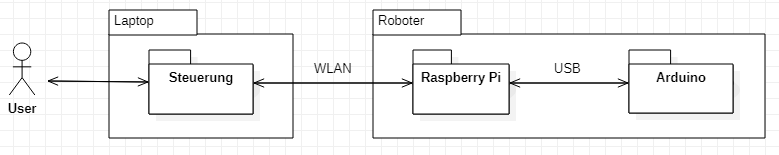
\includegraphics[width=9cm]{img/Gesamtsystem.PNG}
		\caption{Gesamtxberblick des Systems}
		\label{Gesamt zusammenhang}
	\end{figure}
	Die Abbildung \ref{Gesamt zusammenhang} zeigt das System, welches auf mehrere Komponenten basiert. Innerhalb des Systems wird eine Software eingesetzt, die auf dem Robot Operating System (ROS) basiert. Diese Software läuft verteilt auf den Komponenten Laptop, Raspberry PI und Arduino, wie hier in Abbildung \ref{Gesamt zusammenhang} zu sehen. \\
	
	Beginnend werden wir mit der Komponente Laptop. Sie ist dazu da, dem User die Steuerung des Roboters zu ermöglichen. Die Steuerung kann erst erfolgen, wenn auf dem Raspberry PI ein Accespoint geöffnet, mit dem sich der Laptop - der Nutzer letztendlich - via WLAN verbindet.\\
	Innerhalb der anderen Komponente Roboter - unser rosBerry - befindet sich die beiden Hardware-Elemente Raspberry PI und ein Arduino. Der Arduino wird durch ein USB Kabel mit der Raspberry PI verbunden. Dadurch wird eine Kommunikation ermöglicht, in dem der Arduino den Raspberry PI in Zeitabständen mit Sensordaten versorgt.\\
	An dieser Stelle ist anzumerken, dass weitere Hardware verwendet wird, die im Kapitel Hardwareaufbau näher vorgestellt wird.
	
	%----------------------------------------------------------------
	\subsection{ROS Knoten Software Architektur}%heike
	%grobstruktur,  nodes topics und all das was es schon als text gibt
	In diesem Kapitel stellen wir euch die Software des Roboters vor. Der dazugehörige Sourcecode finden sie auf github.com/Wifi-cable/Robotic\_AI\_student\_project. An dieser Stelle möchten wir nochmals darauf hinweisen, dass das Repository von Tiziano Fiorenzani geklont wurde. Die Dokumentation seines Projektes finden sie unter folgende Verlinkung zu Youtube https://youtu.be/iLiI\_IredhI.
	
	% Das Bild später bei Existenz aller Knoten aktualisieren.
	\begin{figure}[!ht] 
		\centering
		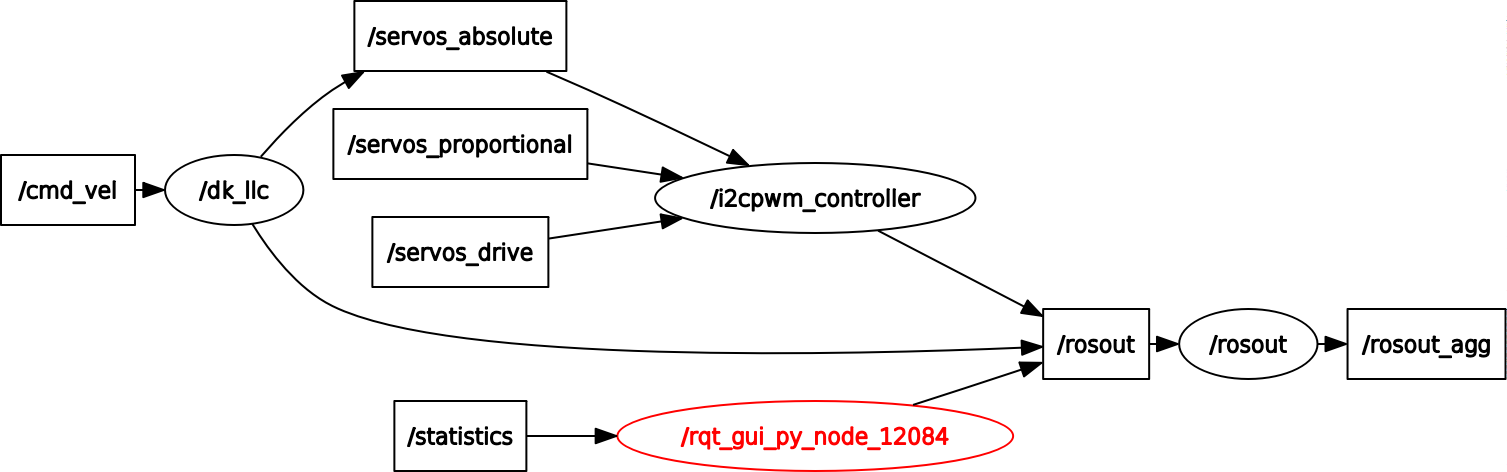
\includegraphics[width=9cm]{img/rosgraph.png}
		\caption{Übersicht der ROS Elemente}
		\label{rosgraph}
	\end{figure}
	
	Treu nach den Prinzipien von ROS besteht die Software aus vielen ROS Nodes, welche als Oval dargestellt werden. 
	Jeder Node erledigt kleine Aufgaben und kann als Subscriber und/oder Publisher fungieren. Die Kommunikation zwischen Subscriber und Publisher erfolgt durch ROS Messages (Nachrichten). Diese werden durch verschiedene Topics - werden als Rechteck dargestellt - kommuniziert. Die Topics kann man als Kanäle für Nachrichten betrachten.
	
	Folgende Nodes befinden sich im Softwaresystem:
	\begin{itemize}
		\item /rosout (Master)
		\item /teleop\_twist\_keyboard (Fernsteuerung)
		\item /donkey\_llc (Hardwarenahe Steuerung)
		\item /ic2pwm\_board\_node (Bibliothek und Node zum Ansprechen des I2C Protokolls und deren Verbindung mit ROS)
		\item serial\_node.py (Publisher der Utraschallsensordaten
	\end{itemize}
	
	Die zuvor genannten Nodes sind durch Topics miteinander verbunden und tauschen untereinander Nachrichten aus. Folgende Topics befinden sich im Softwaresystem:
	\begin{itemize}
		\item /cmd\_vel (comand velocity, die Beschleunigungssteuerung)
		\item /servos\_absolute (Steuerung des Servos mit absoluten Impulsstart- und Stoppwerten)
		\item /servos\_proportional (Motorsteuerung für Geschwindigkeit Steuerung des Servos in ihrem Bewegungsbereich)
		\item /servos\_drive (Lenken, Umwandlung der Berechnungen von Linear- und Winkeldaten in Servoantriebsdaten)
		\item /rosout (Standard ROS Output)
		\item /rangeMsg\_topic (Datenübertragung der Ultraschallsensordaten)
	\end{itemize}
	
	%----------------------------------------------------------------
	% Je nach Formatierung wird dies verändert werden dürfen und der pagebreak entfernt
	\pagebreak
	\subsubsection{Launch Reihenfolge}%heike
	
	Dieses Kapitel ist eine Einleitung zum Starten der ROS Nodes und die hierbei zu beachtenden Punkten.
	
	% Weitere Knoten werden noch folgen
	\begin{lstlisting}[label={list:first},caption=Sample rosBash code.]
	# Network ubiquityrobot03B
	# connect via SSH
	ssh ubuntu@10.42.0.1
	# enter password
	
	# 1. Console - on Raspberry PI
	# Login via SSH
	cd catkin_ws/Robotic_AI_student_project/
	source devel/setup.bash
	rosrun i2cpwm_board i2cpwm_board
	
	# 2. Console - on Raspberry PI
	# Login via SSH
	cd catkin_ws/Robotic_AI_student_project/
	source devel/setup.bash
	rosrun donkey_car low_level_control.py
	
	# 3. Console - on Laptop 
	export ROS_MASTER_URI=http://ubiquityrobot.local:11311
	export ROS_IP=$(hostname -I)
	cd catkin_ws/Robotic_AI_student_project/
	source devel/setup.bash
	rosrun teleop_twist_keyboard teleop_twist_keyboard.py
	
	# 4. Console - on Raspberry PI
	# Login via SSH
	rosrun rosserial_python serial_node.py /dev/ttyACM0
	
	# 5. Console - on Laptop
	export ROS_MASTER_URI=http://ubiquityrobot.local:11311
	export ROS_IP=$(hostname -I)
	rostopic echo rangeMsg_topic
	\end{lstlisting}
	%----------------------------------------------------------------
	
	\section{Praktische Projekt Durchführung}
	
	%----------------------------------------------------------------
	
	\subsection{Hardwareaufbau}%Heike 
	In diesem Kapitel beschreiben wir den Hardwareaufbau des rosBerry. Hierfür werden wir die einzelnen verwendeten Hardwarekomponenten - deren Modell und Funktion - vorstellen.
	
	Zuerst bilden wir die Verbindungen der Hardwarekomponenten untereinander ab, wie in Abbildung \ref{Hardwarekomponenten} zu sehen.
	
	\begin{figure}[!ht]
		\centering
		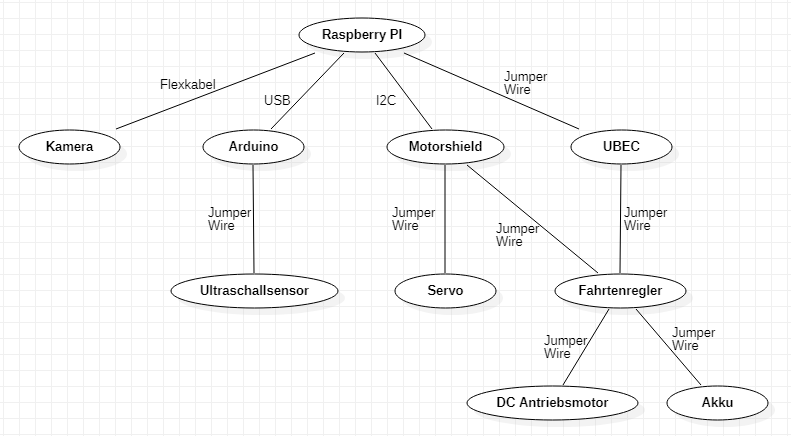
\includegraphics[width=9cm]{img/Hardwarekomponenten.PNG}
		\caption{Verbindungen der Hardwarekomponenten im rosBerry}
		\label{Hardwarekomponenten}
	\end{figure}
	
	Wie aus der Abbildung \ref{Hardwarekomponenten} zu erkennen, ist die meiste Hardware mit Jumper Wire verbunden. Ausnahmen der Anschlüsse bilden die Verbindungen des Raspberry PIs zur Kamera (Flexkabel), zum Arduino (USB) und zum Motorschield (I2C).\\
	
	Als Nächstes wird rosBerry mit den Hardwaremodellen vorgestellt.
	\\
	\begin{figure}[!ht]
		\centering
		\includegraphics[width=9cm]{img/RosBerryGesamt.png}
		\caption{Gerüst rosBerry}
		\label{rosBerryGesamt}
	\end{figure}
	
	Die verwendete Hardware ist in Abbildung \ref{rosBerryGesamt} mit Nummern versehen. Auf jede dieser Nummern wird referenziert und die Hardware mit Modell und Funktion aufgelistet.
	
	\begin{enumerate}
		\item Der DC Antriebsmotor - Modell Tamiya Mabuchi RS 540 SH - steuert alle vier Reifen des rosBerry an. Ohne ihn wird der Roboter nicht in Bewegung kommen.
		\item Neben dem DC Antriebsmotor befindet sich ein Fahrtenregler, Model BORSTI 1/10 BRUSHED-ESC 45A. Dieser erhält vom Motorshield ein PMW Signal, welches er verstärkt. Das verstärkte PWM Signal wird anschließend in Geschwindigkeit umgesetzt und an den DC Antriebsmotor weitergeleitet.
		\item Der UBEC - Modell HWBEC Hobbywing 3A 5V 6V max 5A - wird eingebaut, um den Raspberry PI mit 5 Volt zu versorgen. Ohne den UBEC würde der Raspberry PI aufgrund der höheren elektrischen Spannung beschädigt werden.
		\item Der Servo - Modell Amewi AMX Racing 4806HB - bekommt vom Motorshield ein PWM Signal übermittelt. Nach dem PWM Signal richten sich die beiden Reifen aus und ermöglichen eine Fahrtrichtung. Dadurch ist rosBerry in der Lage rechts/links Kurven sowie gerade aus zu fahren.
		\item Der Akku dient dazu, die Stromversorgung des Roboters zu sichern. Dieser liefert 7 Volt und versorgt die weitere Hardware mit Strom.
		\item Der Motorschield - Modell Adafruit 16-Channel 12-bit PWM/Servo Driver-I2C interface PCA9685 - wird für die Geschwindigkeit und die Richtung der Reifen eingesetzt. Hierzu erzeugt der Motorshield zwei PWM Signale. Das 1. PWM Signal wird an den Servo übermittelt, um den Servo in die gewünschte Position einzustellen. Das 2. PWM Signal wird erzeugt und zum Fahrtenregler gesendet. Dieses wird zur Einstellung der Geschwindigkeit verwendet.
		\item Der Raspberry PI 3.b+ ist das Herzstück des rosBerries. Auf ihn läuft zum einem ROS und zum anderen die Software des Roboters, welche in Kapitel ROS Knoten Software Architektur vorgestellt wurde. 
		Über eine I2C-Schnittstelle werden Daten an den Motorshield übertragen. Die Daten geben an wie das PWM Signal auszusehen hat.
		\item Der Arduino UNO REV 3 steuert einen Ultraschallsensor an und erzeugt einen ROS Knoten (Publisher).
		Innerhalb des Programm wird das Signal des Sensors in Meter umgewandelt und in eine Range Message gespeichert. Die Range Message namens rangeMsg wird an das Topic rangeMsg\_topic übermittelt. Ein Subscriber - der auf dem Raspberry PI läuft - subscribed das Topic und erhält regelmäßig Sensordaten über die Reichweite.
		
		\begin{figure}[!ht]
			\centering
			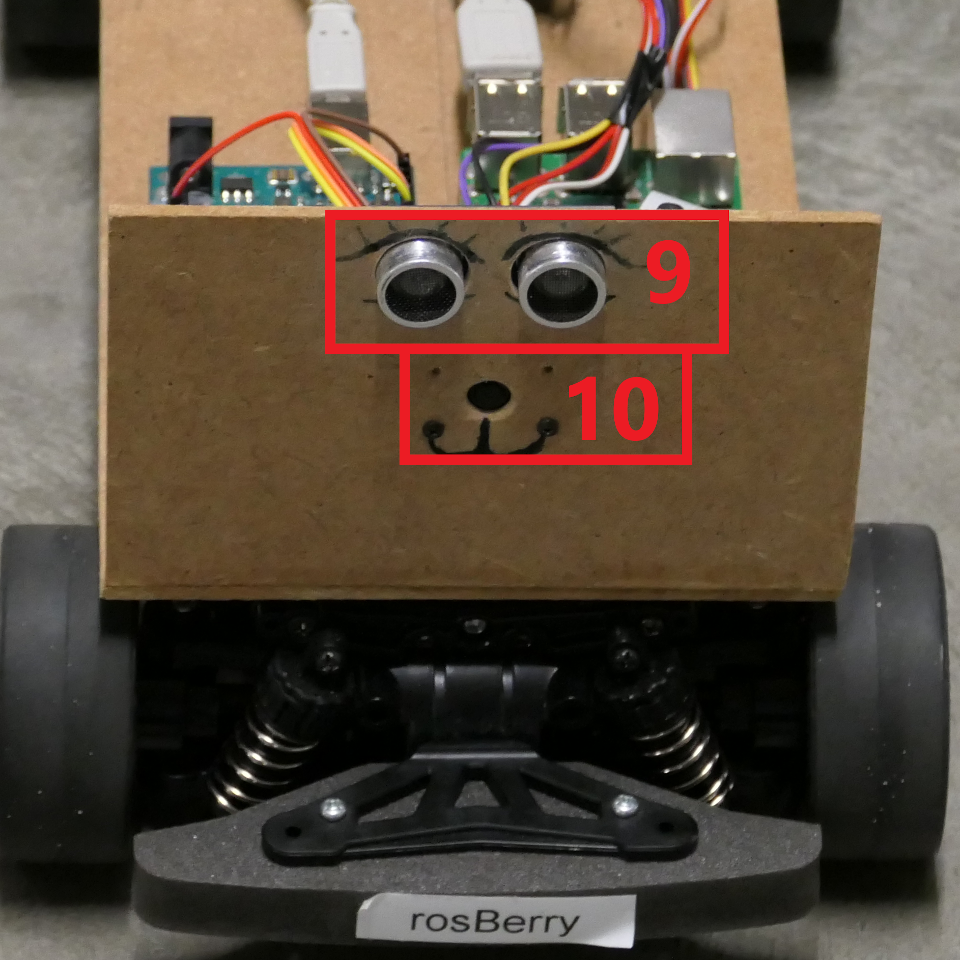
\includegraphics[width=5.5cm]{img/RosBerryWeitere.png}
			\caption{Weitere Hardwareelemente}
			\label{rosBerryWeitere}
		\end{figure}
		\item Der Ultraschallsensor - Modell HC-SR04 - wird zum rechtzeitigen erkennen eines kommenden Hindernisses eingesetzt. Dieser hat eine maximale Reichweite von 4 Meter, jedoch haben wir uns für das Projekt auf eine Reichweite von 2 Meter geeinigt.
		Alles x Sekunden sendet dieser ein Signal und verarbeitet dieses.
		\item Die Kamera - Modell 5 MP - ist durch ein Flexkabel an den Raspberry PI angeschlossen. Diese versorgt eine KI mit Bildern, welche einen Marker sucht und findet.
	\end{enumerate}
	
	%----------------------------------------------------------------
	
	
	\section{Autonomes verhalten durch Künstliche Intelligenz  }	%mary
	
	Ziel des KI Teil des Projekts besteht darin dem Roboter Beizubringen  einem Optischen Marker zu folgen. Dazu muss er erst einmal das Symbol erkennen, dann herausfinden in welche Richtung sich der Marker befindet. Danach erst kann er auf den Marker zufahren. \\ 
	
	Der schwierigste Teil der Aufgabe besteht darin den Marker zuverlässig in unterschiedlichen Umgebungen zu erkennen. 
	
	\subsection{Erster Ansatz für das Neuronale Netz}	%steffen ? mary?
	%netzaufbau am anfang
	\subsubsection{Este Auswertung der Ergebnisse}	%steffen? 
	%wiso war das scheisse
	\subsection{Schritte zur Verbesserungen der Erkennungsrate} %mary
	%was haben wir dann gemacht 
	\subsection{Anwendung des Trainingsmodells } %steffen +mary
	%bild teilen
	%bild analysieren
	%  entscheidung treffen, rechts, links geradeaus oder rückwärtz
	\subsection {Auswertung des verhalten des Roboters}	% mary? %steffen? %heike?
	%macht er irgendwas sinnvolles? ist er klüger als eine eintagsfliege
	
	\begin{comment}	%  how-to formeln 
	\begin{equation}
	a+b=\gamma\label{eq}
	\end{equation}
	\end{comment}
	\begin{comment}
	\paragraph{Positioning Figures and Tables} 
	Use the abbreviation 
	``Fig.~\ref{fig}'', even at the beginning of a sentence.
	
	\begin{table}[htbp]
	\caption{Table Type Styles}
	\begin{center}
	\begin{tabular}{|c|c|c|c|}
	\hline
	\textbf{Table}&\multicolumn{3}{|c|}{\textbf{Table Column Head}} \\
	\cline{2-4} 
	\textbf{Head} & \textbf{\textit{Table column subhead}}& \textbf{\textit{Subhead}}& \textbf{\textit{Subhead}} \\
	\hline
	copy& More table copy$^{\mathrm{a}}$& &  \\
	\hline
	\multicolumn{4}{l}{$^{\mathrm{a}}$Sample of a Table footnote.}
	\end{tabular}
	\label{tab1}
	\end{center}
	\end{table}
	
	\begin{figure}[htbp]
	\centerline{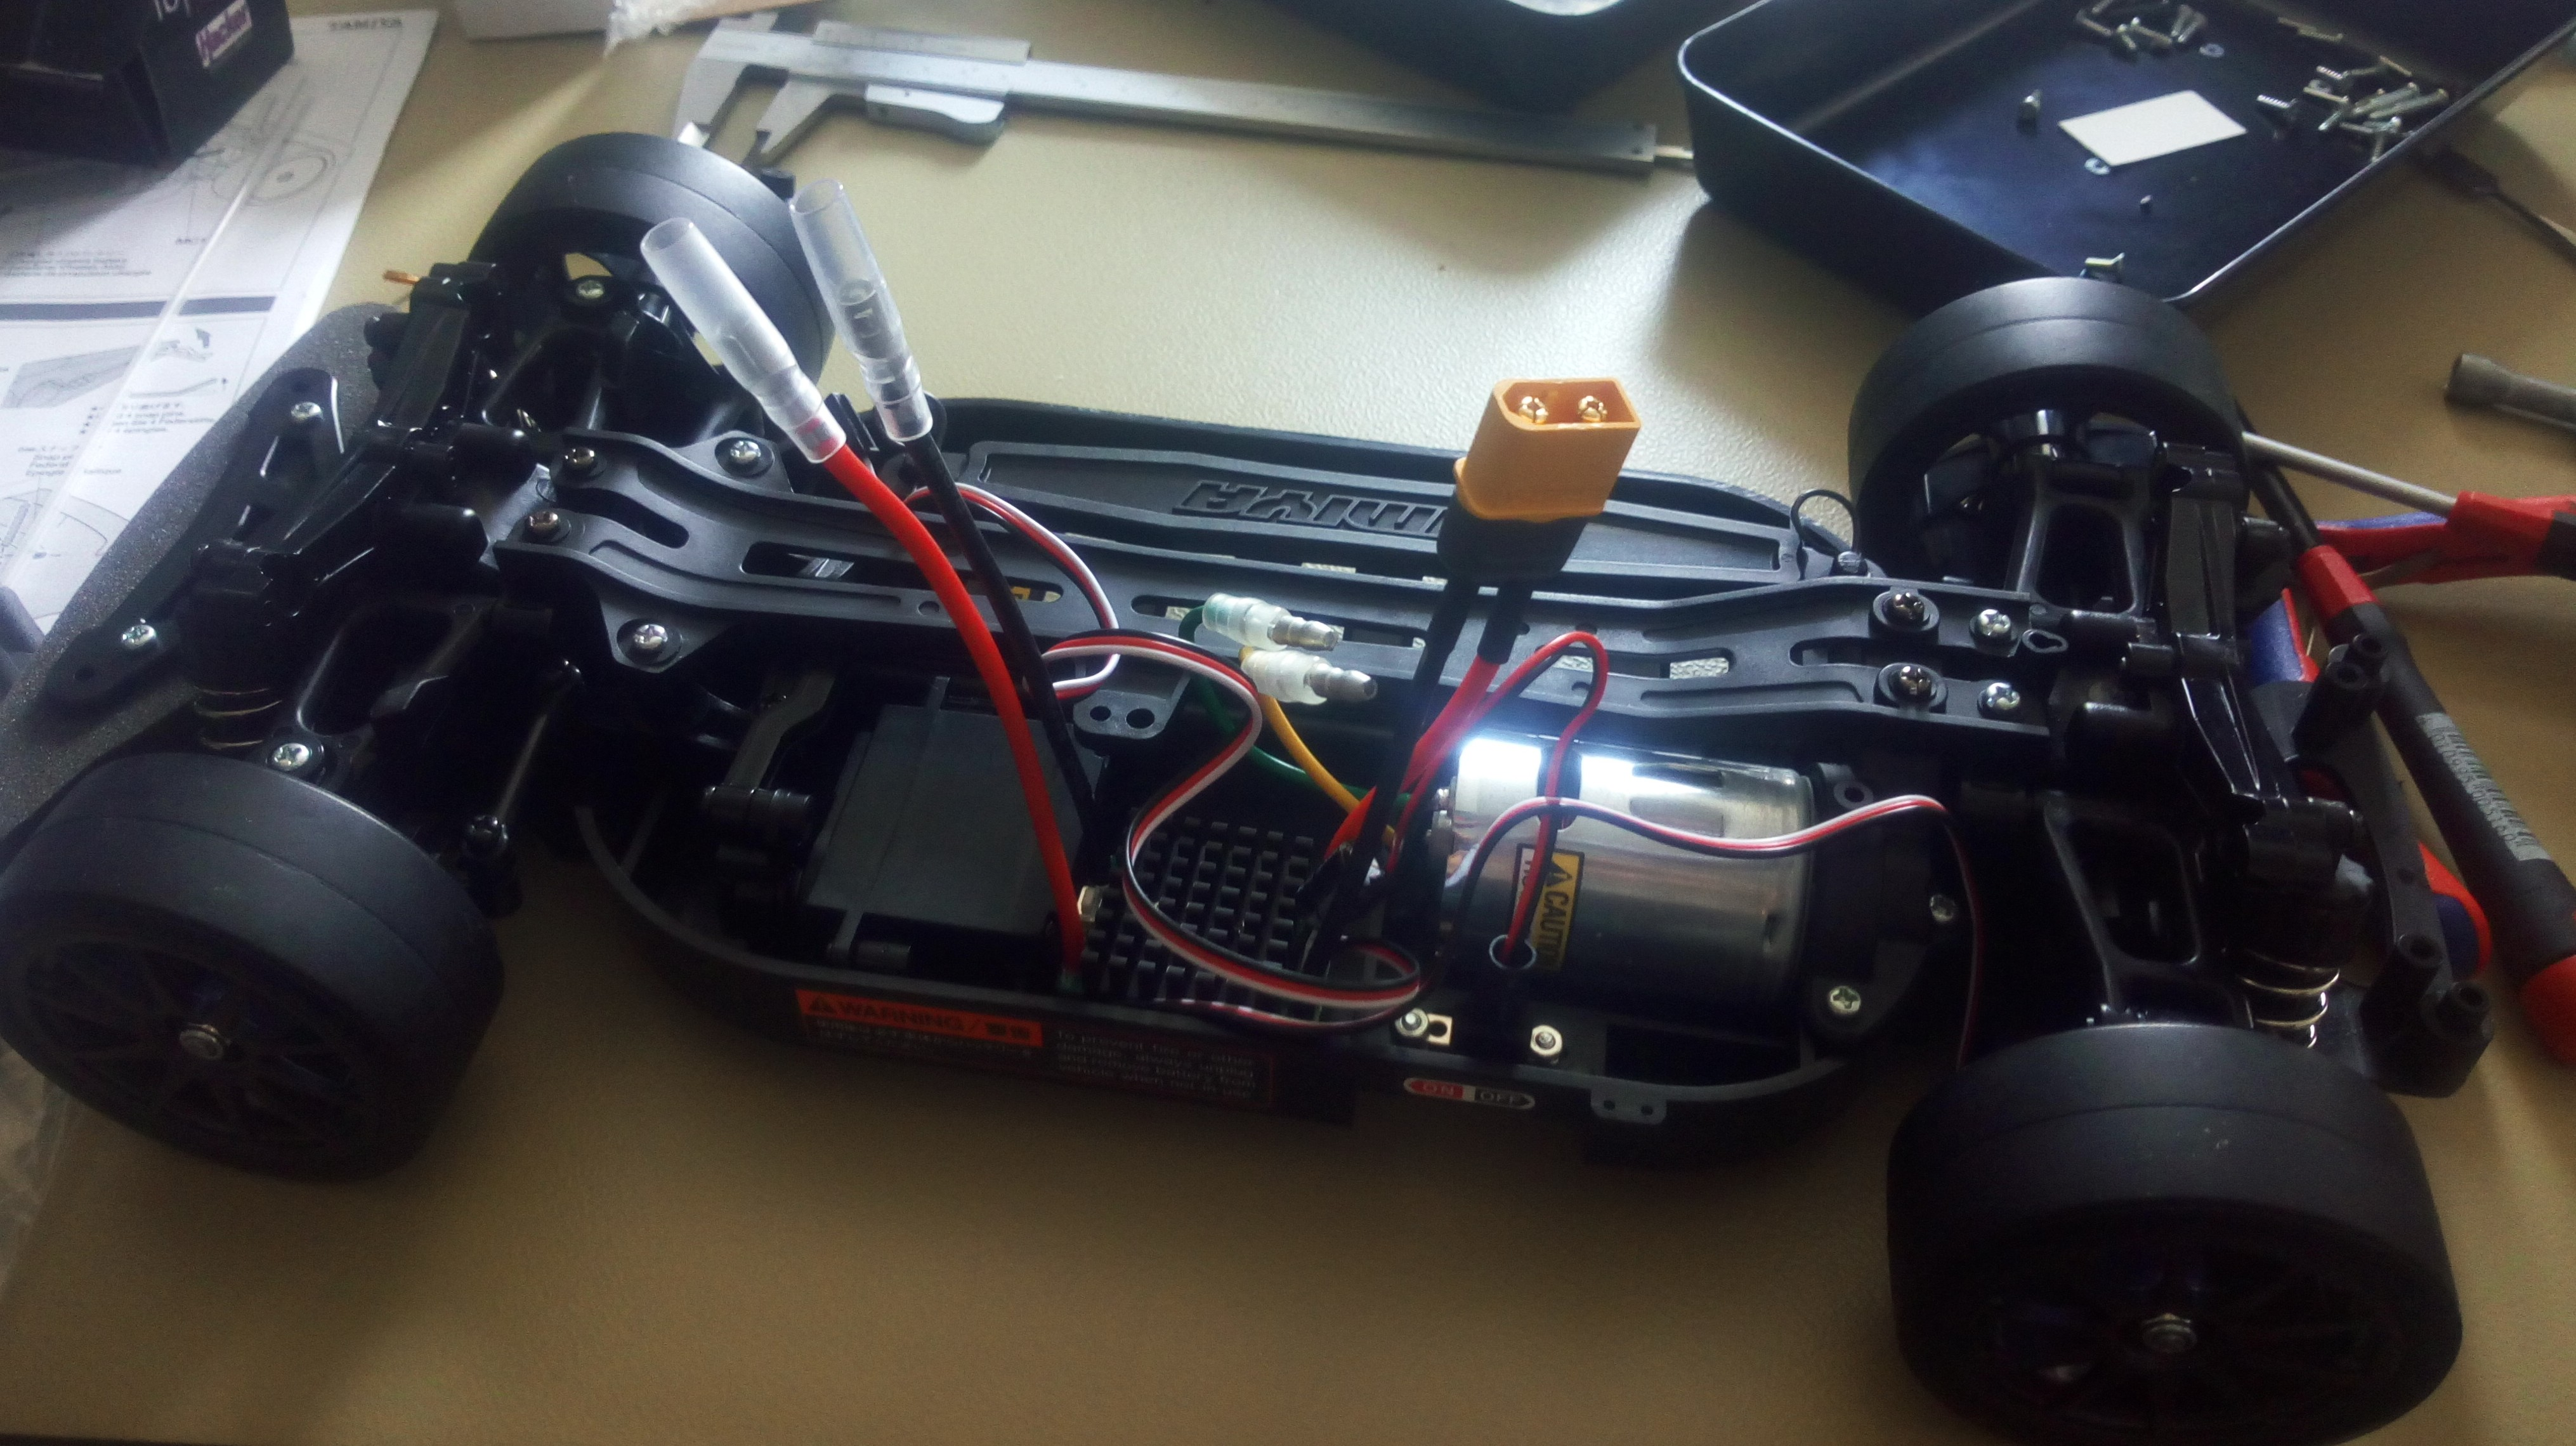
\includegraphics{img/car_body.jpg}}
	\caption{Example of a figure caption.}
	\label{fig}
	\end{figure}
	\end{comment}
	
	
	%\section*{Acknowledgment}
	% wollen wir unseren profs danken, weil mehr GPU und RAM? 
	
	% wissenschaftliche zitate gehen so \cite{b1}. 
	
	
	%Francis X. Govers - Artificial Intelligence for Robotics-Packt Publishing (2018).pdf
	\begin{thebibliography}{00}
		\bibitem{b1}Francis X. Govers , ` Artificial Intelligence for Robotics,''Packt Publishing ,2018
		
	\end{thebibliography}
	
	
\end{document}
